\documentclass[tikz,border=6pt]{standalone}
\usepackage{amsmath,amssymb}
\usepackage{xcolor}
\definecolor{accent}{HTML}{A13D2C}
\definecolor{accent2}{HTML}{2B5F6B}
\definecolor{muted}{HTML}{5A564F}
\definecolor{panel}{HTML}{F8F6F0}
\definecolor{linecol}{HTML}{D8D2C4}
\definecolor{astroblue}{HTML}{1B4F72}
\definecolor{sunyellow}{HTML}{E8A33D}
\definecolor{colthree}{RGB}{60,140,80}
\usetikzlibrary{calc,arrows.meta,plotmarks}
\IfFileExists{results/ch12/lane_emden_n3.dat}{\def\datadir{results/ch12/}}{\def\datadir{../results/ch12/}}
\begin{document}
% Isothermal sphere: log10(rho/rho_c) against log10 xi (cluster data), with the singular solution 2/xi^2 dashed.
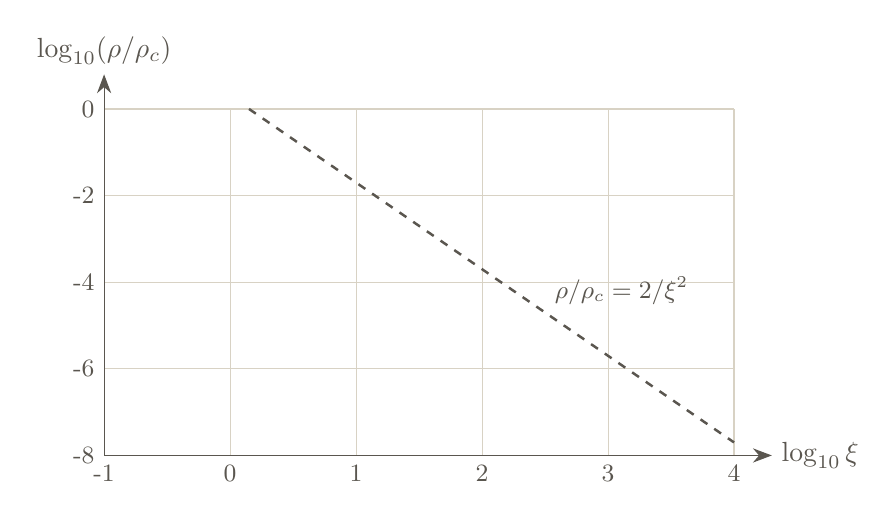
\begin{tikzpicture}[x=1.6cm,y=0.55cm, >={Stealth[length=2.4mm]}]
  \draw[linecol] (-1,-8) grid[xstep=1,ystep=2] (4,0);
  \draw[->, muted] (-1,-8) -- (4.3,-8) node[right] {$\log_{10}\xi$};
  \draw[->, muted] (-1,-8) -- (-1,0.8) node[above] {$\log_{10}(\rho/\rho_c)$};
  \foreach \x in {-1,0,1,2,3,4} \node[below, muted] at (\x,-8) {\small \x};
  \foreach \y in {-8,-6,-4,-2,0} \node[left, muted] at (-1,\y) {\small \y};
  \draw[muted, dashed, line width=0.9pt, domain=0.15:4] plot (\x, {log10(2) - 2*\x});
  \draw[astroblue, line width=1.2pt] plot file {\datadir isothermal.dat};
  \node[muted, right] at (2.5,-4.2) {\small $\rho/\rho_c=2/\xi^2$};
\end{tikzpicture}
\end{document}
